\chapter{Future work}

This chapter briefly describes required steps for the sensor to be able to fly on-board PW-Sat2.

\section{Qualification model}
    Firstly, the sensor will be implemented on PC-104 factor board, with all final components and procedures. This model is during designing (figure \ref{PLD_BOARD}).

    \begin{figure}[H]
        \centering
        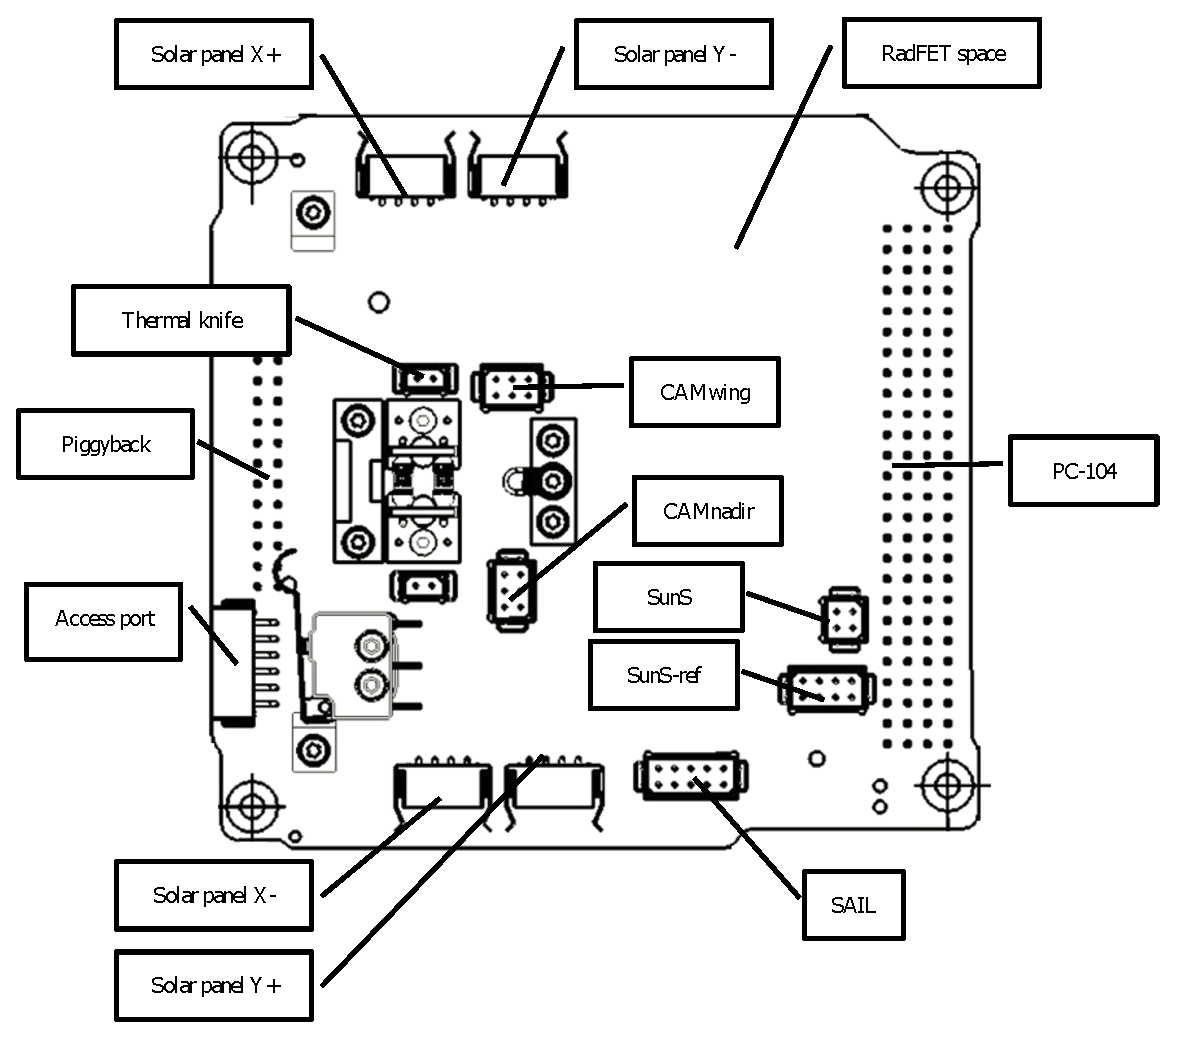
\includegraphics[width=0.7\paperwidth]{img/08/PC104pldBoard.eps}
        \caption{PLD board with connector and space designed for RadFET}
        \label{PLD_BOARD}
    \end{figure}


    On this model all software tests (on flat-sat) will be done, as well as final confirmation of design (thermal, radiation and time-stability tests). This board will qualify sensor design and software for flight use.

\section{Flight model}
    At the end final flight version of the PCB will be manufactured. In the principle, it should be identical to Qualification Model, but handling procedures will be much more strict. Additionally, on flight model only thermal calibration will be made, without further stress-testing. During integration, final version of the sensor on PC104-board will be placed on electronics stack inside PW-Sat2.
